\documentclass[a4paper]{article}
\usepackage[utf8]{inputenc}
\usepackage[english]{babel}
\usepackage{pdfpages, titling}
\usepackage{array, float}
\usepackage{cite, tablefootnote}
\usepackage{graphicx, caption}
\usepackage{listings}
\usepackage{color}
\usepackage{mathtools, braket}
\usepackage{amssymb}
\usepackage[nottoc]{tocbibind} % references in the toc
\usepackage{subcaption}
\usepackage{textcomp}
\usepackage{minted}
\usepackage[hidelinks]{hyperref}
\graphicspath{{Pictures/}} % Specifies the directory where pictures are stored

\newcommand{\vect}[1]{\boldsymbol{#1}}
\newcommand{\subtitle}[1]{
  \posttitle{
    \par\end{center}
    \begin{center}\large#1\end{center}
    \vskip0.5em}
}
\lstset{frame=tb,
  language=Java,
  aboveskip=3mm,
  belowskip=3mm,
  showstringspaces=false,
  columns=flexible,
  basicstyle={\small\ttfamily},
  numbers=none,
  breaklines=true,
  breakatwhitespace=true,
  tabsize=3
}

\author{Jaro Camphuijsen (6042473) and Rahiel Kasim (10447539)}
\title{Scientific Computing II}
\subtitle{The Return of the SciCoPyth}

\begin{document}
\maketitle

\tableofcontents

\section{Diffusion Limited Aggregation}
Diffusion Limited Aggregation (DLA) considers diffusing particles that that can stick to a certain structure and thereby expand the structure. Because we are dealing with diffusion we should solve the diffusion equation at each growth step to calculate the new concentration of particles. 

\begin{equation}
\frac{\partial \phi (r,t)}{\partial  t} = D \nabla ^2 \phi (r,t)
\label{eq:diff}
\end{equation}

Because the growth of such a structure (e.g. a coral or mineral structure) is on a very long timescale and the structure growth per step is very small we can assume the diffusion reaches equilibrium before the next step and we can solve the time independent diffusion equation. 

The update scheme of a growth simulation of a certain number of \mintinline{python}{steps} is given in the following pseudo code snippet:

\begin{minted}[]{python}
def grow(eta, omega, steps):
    for n in range(steps):
        nutLattice = SOR(omega, objLattice)
        objLattice = grow_step(eta, nutLattice)
\end{minted}

Here we have the nutrient lattice \mintinline{python}{nutLattice} which is updated each time step by the \mintinline{python}{SOR} function and contains the nutrient concentration at each cell, it uses the object lattice \mintinline{python}{objLattice} for its boundary conditions. The object lattice is updated using the \mintinline{python}{grow_step} function to calculate the probability for each cell to become part of the structure from the nutrient concentration in the cell. 

To simulate the growth we define two different cell states: a cell can be part of the structure or it can be empty. Each step we determine all grow candidates. For a cell to be a grow candidate it must be empty and has one of his neighbours be part of the structure. Each candidate has the following probability to switch it state from empty to be part of the structure:

\begin{equation}\label{eq:grow_prob}
    p_g (i,j) = \frac{c_{i,j}^{\eta}}{\sum_{\text{candidates}} c_{i,j}^{\eta}}
\end{equation}

For the calculation of the time independent diffusion equation we use the successive over-relaxation (SOR) function from the last assignment. In the previous assignment \cite{scico1} we also optimized the relaxation parameter $\omega$, however the optimal value of $\omega$ depends on the boundary values of the domain. These were fixed in the simple example of the previous exercise but since we have a growing object this time, the value of $\omega$ should in principle be optimized every time the structure has grown a bit. This to computationally demanding to be of any use. 

When we do a simulation with a growing parameter $0 < \eta < 1$ we get a problem using the SOR calculation. Due to the over relaxation it is possible to end up with a small negative concentration. This is no problem for other values of $\eta$, however since the root of a negative number is not defined in our program we end up with an error. To avoid this problem in calculation and because we can not truly optimize $\omega$ which would result in a minor speed improvement anyway, we should set $\omega = 1$ or use under relaxation for all simulations with $0 < \eta < 1$. 

\begin{figure}[ht] 
  \begin{subfigure}[b]{0.5\linewidth}
    \centering
    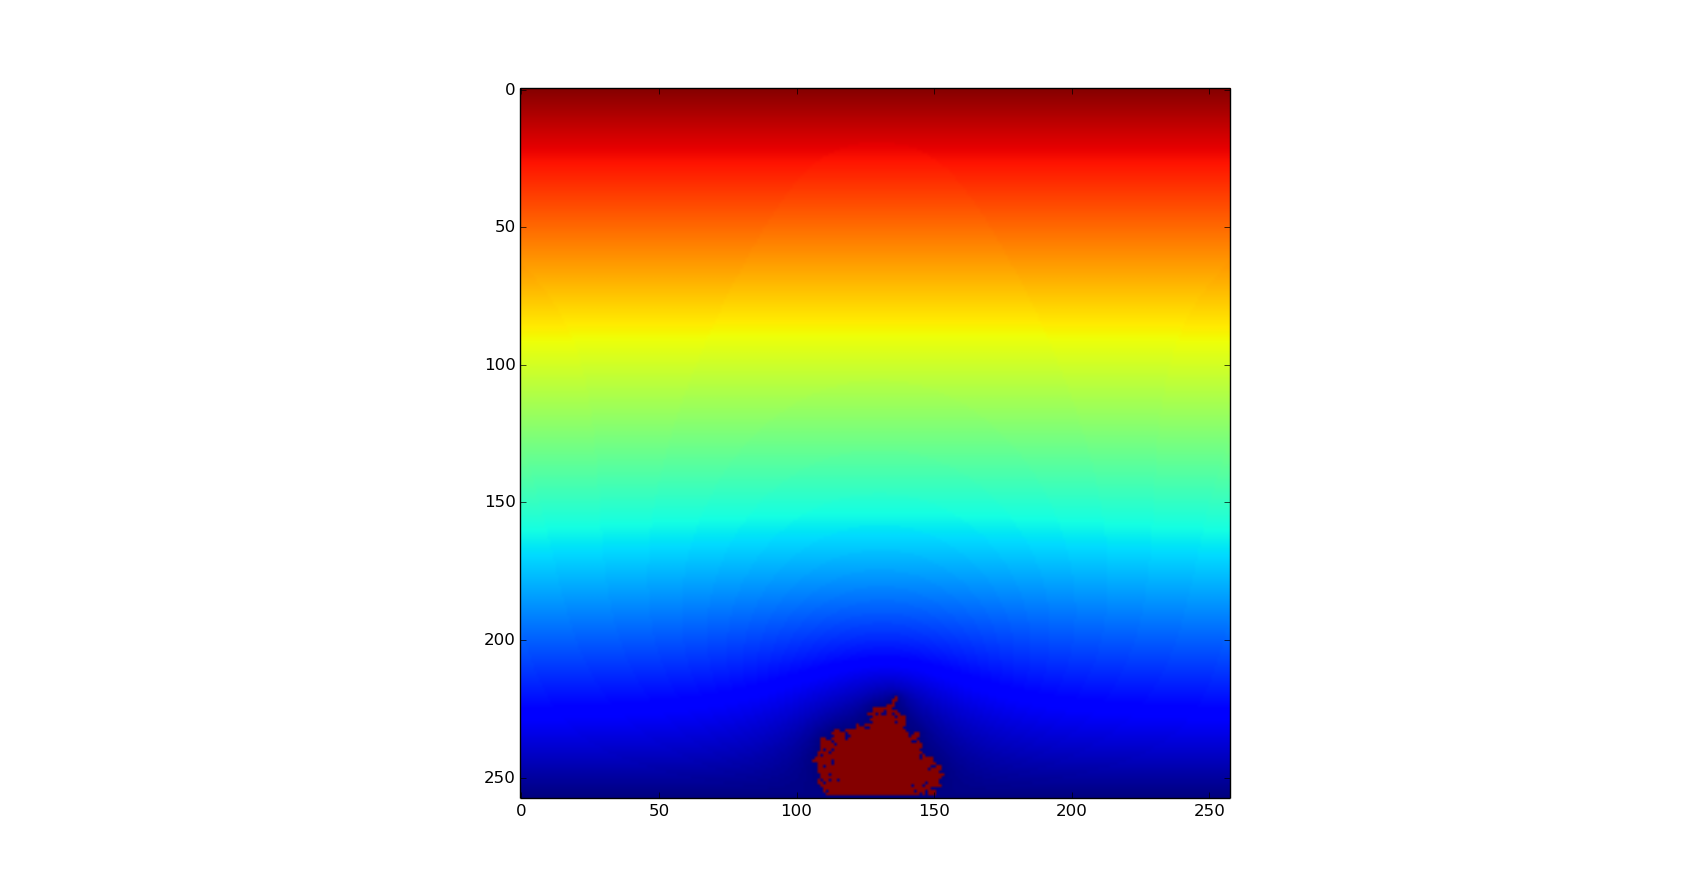
\includegraphics[width=\linewidth, trim={7cm 1.8cm 7cm 1cm},clip]{DLA_eta00.png} 
    \caption{$\eta = 0$} 
    \label{fig:DLA_eta00} 
  \end{subfigure}%% 
  \begin{subfigure}[b]{0.5\linewidth}
    \centering
    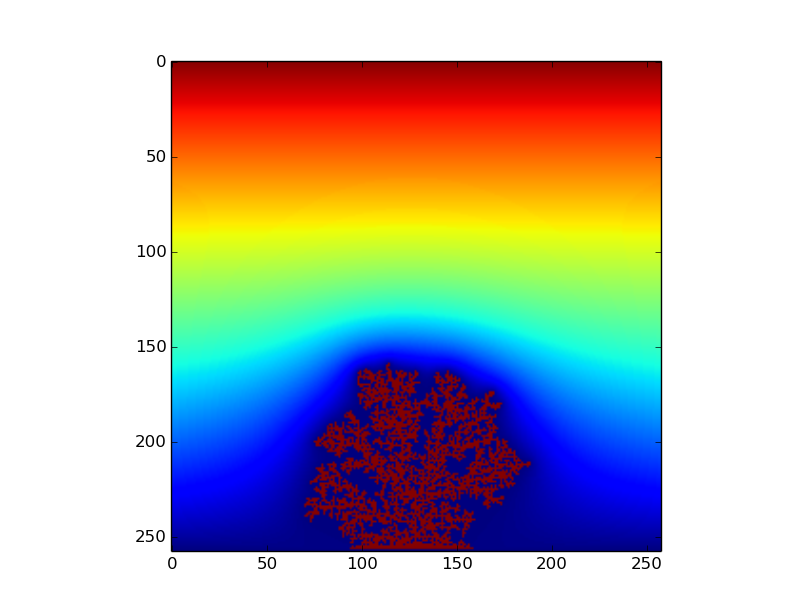
\includegraphics[width=\linewidth, trim={0cm 1cm 0cm 0cm},clip]{DLA_eta05.png} 
    \caption{$\eta = 0.5$} 
    \label{fig:DLA_eta05} 
  \end{subfigure} 
  \begin{subfigure}[b]{0.5\linewidth}
    \centering
    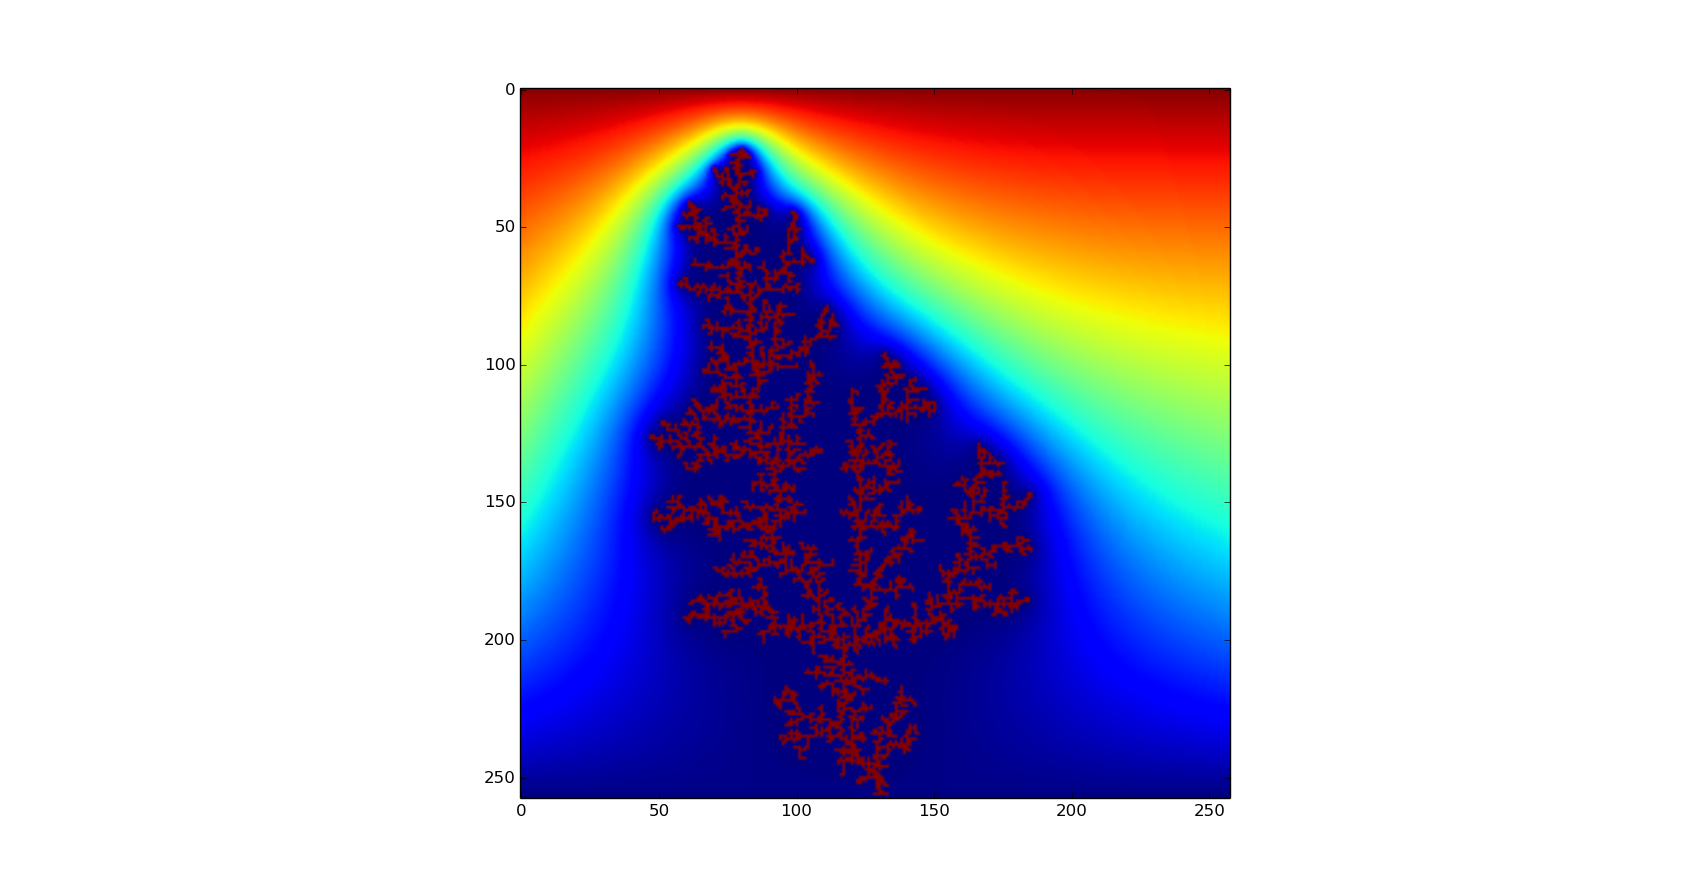
\includegraphics[width=\linewidth, trim={7cm 1.8cm 7cm 1cm},clip]{DLA_eta10.png} 
    \caption{$\eta = 1$} 
    \label{fig:DLA_eta10} 
  \end{subfigure}%% 
  \begin{subfigure}[b]{0.5\linewidth}
    \centering
    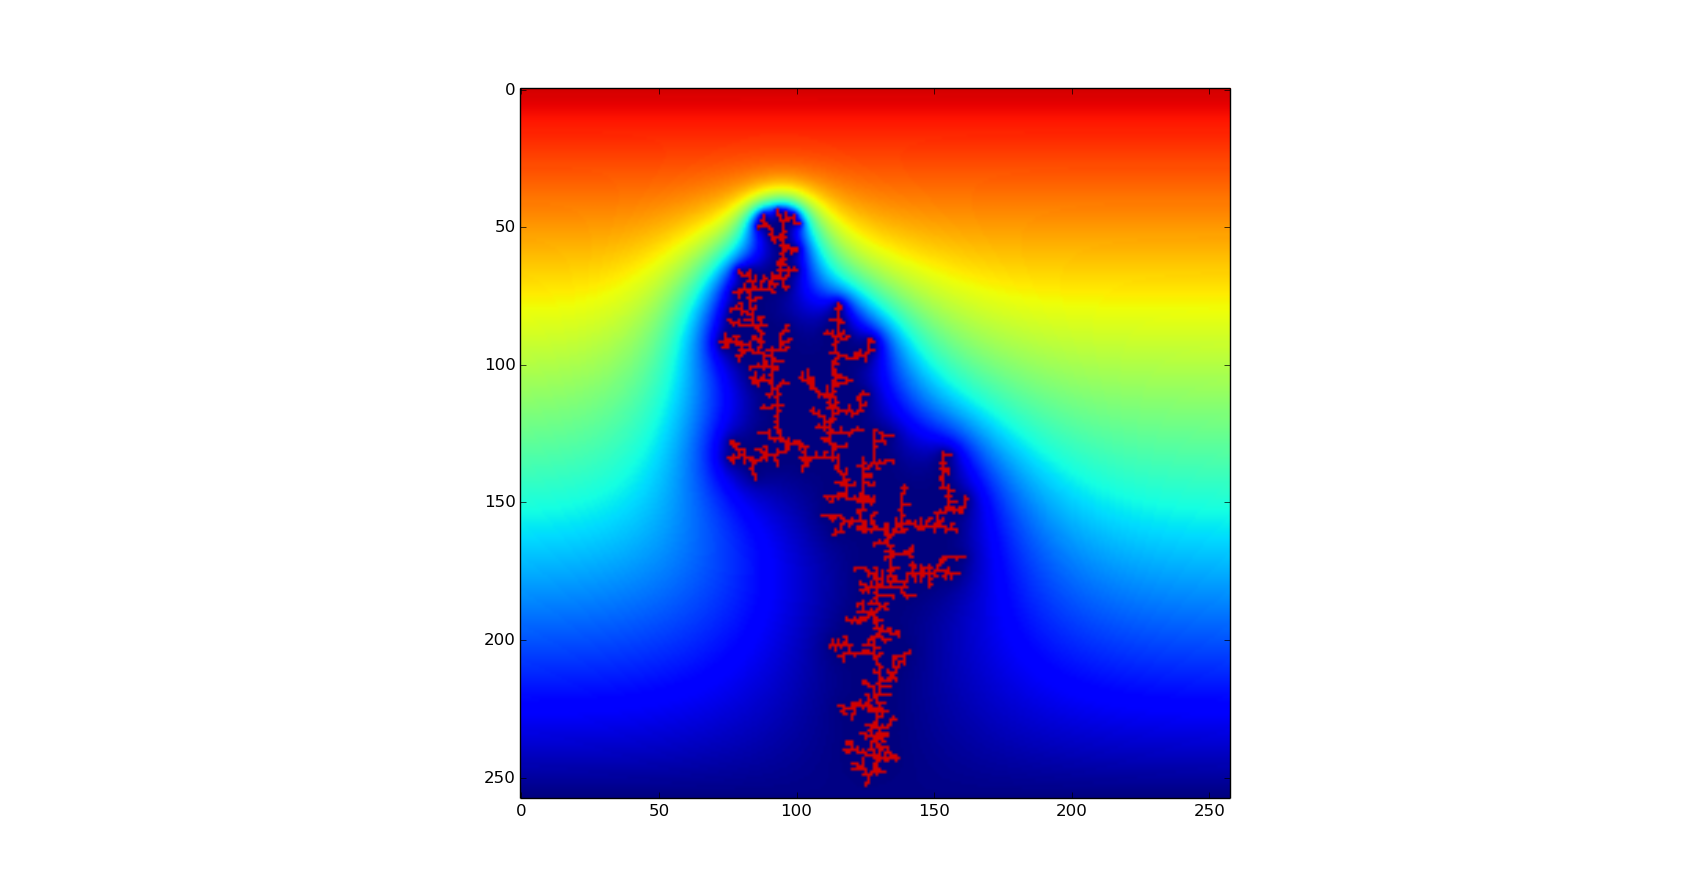
\includegraphics[width=\linewidth, trim={7cm 1.8cm 7cm 1cm},clip]{DLA_eta15.png} 
    \caption{$\eta = 1.5$} 
    \label{fig:DLA_eta15} 
  \end{subfigure}
  \begin{subfigure}[b]{0.5\linewidth}
    \centering
    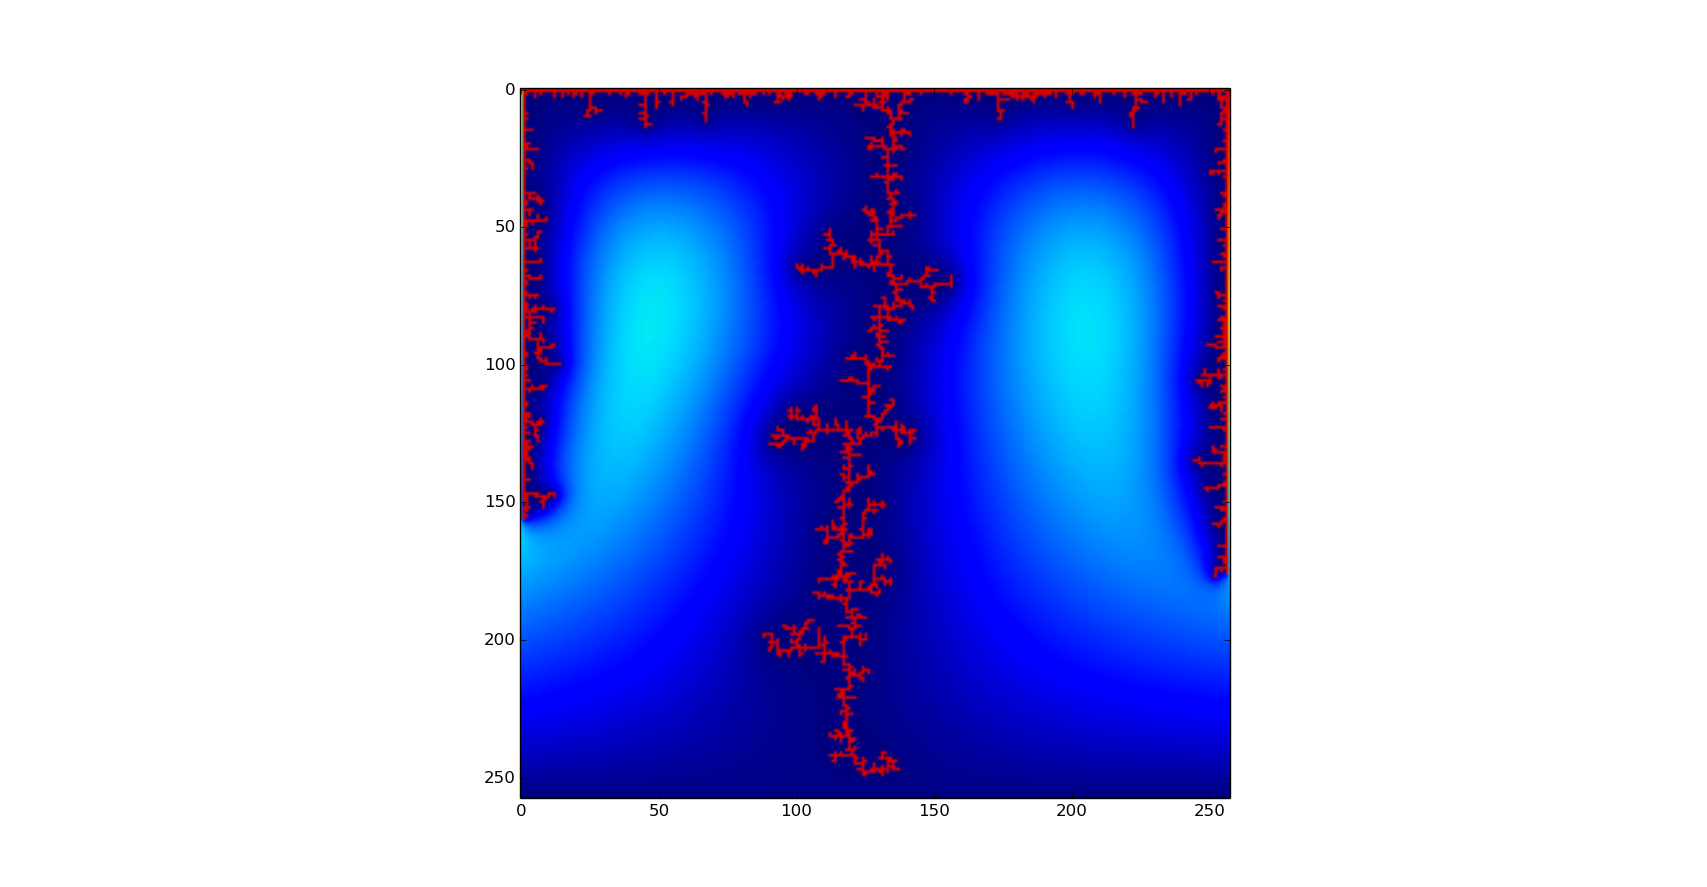
\includegraphics[width=\linewidth, trim={7cm 1.8cm 7cm 1cm},clip]{DLA_eta20.png} 
    \caption{$\eta = 2$} 
    \label{fig:DLA_eta20} 
  \end{subfigure}%% 
  \begin{subfigure}[b]{0.5\linewidth}
    \centering
    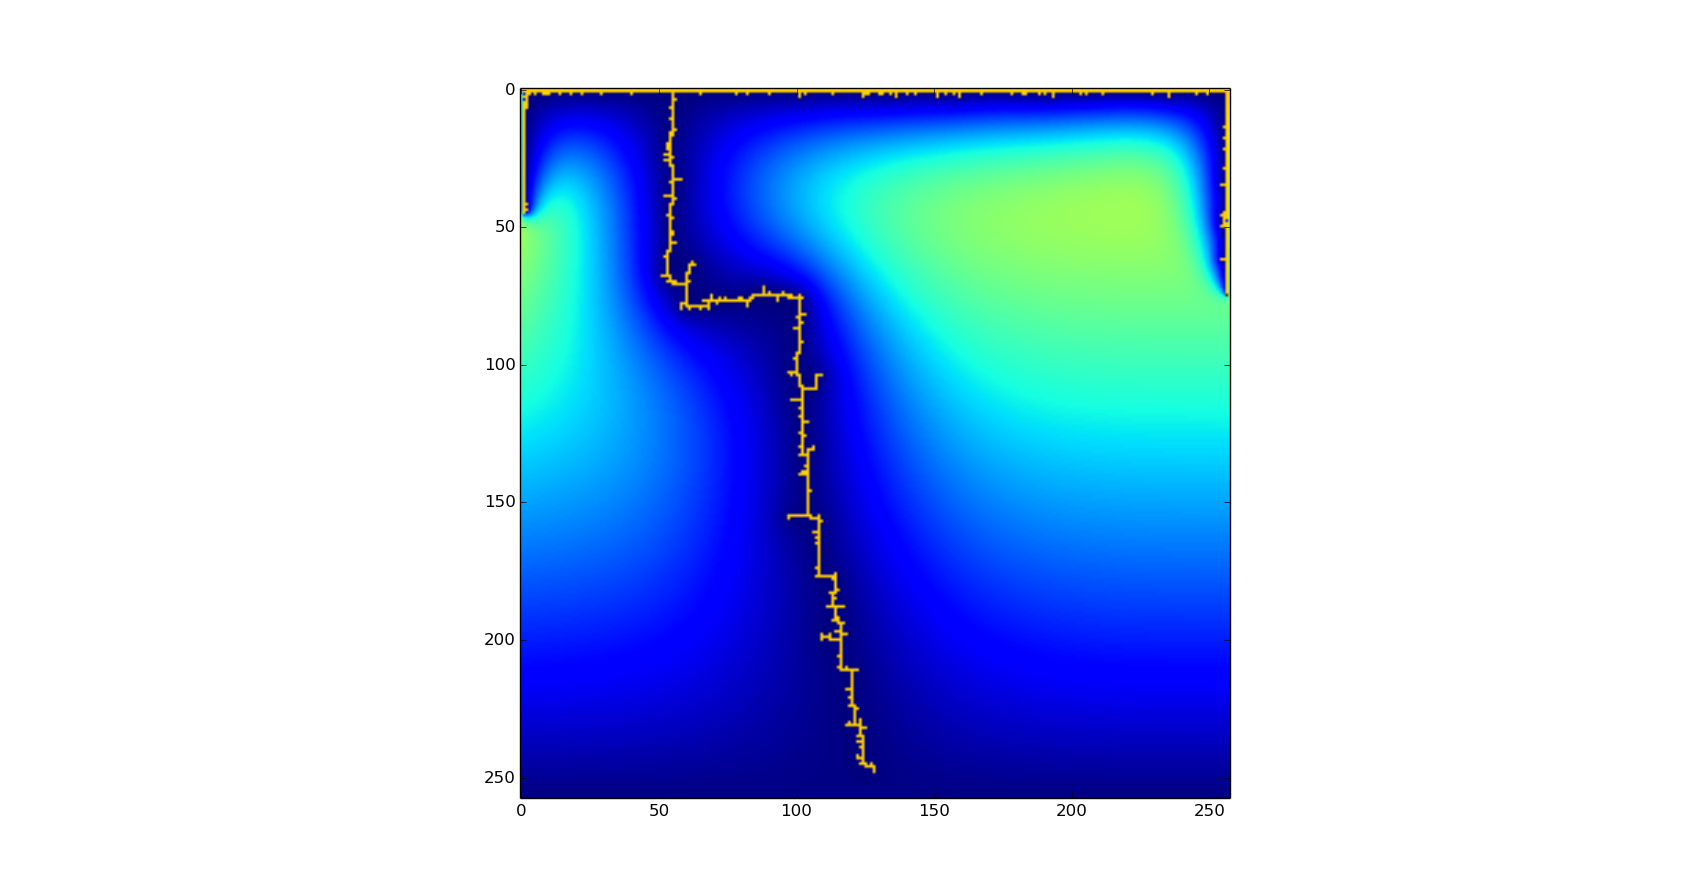
\includegraphics[width=\linewidth, trim={7cm 1.8cm 7cm 1cm},clip]{DLA_eta30.png} 
    \caption{$\eta = 3$} 
    \label{fig:DLA_eta30} 
  \end{subfigure}
  \caption{Diffusion Limited Aggregation for different values of $\eta$}
  \label{fig:DLA_eta} 
\end{figure}

For varying growing parameter $\eta$ we get different structures as shown in figure \ref{fig:DLA_eta}. If we set $\eta$ to zero as in figure \ref{fig:DLA_eta00} we turn off the influence of the nutrient concentration. Each grow candidate has the same probability of growing which results in a circular bulk around the initial point. With increasing $\eta$ the bulk tends to grow towards more expanded structures with normal DLA growth for $\eta = 1$ in figure \ref{fig:DLA_eta10}. If we keep increasing $\eta$ the influence of the nutrient concentration increases and since we have a gradient directed to the top of the domain, the structure will grow more linearly with less pronounced branches. In the case of $\eta = 3$ as seen in figure \ref{fig:DLA_eta30}, the structure is almost completely linear this is because candidate cells at the top of the structure have a much higher probability to become part of the object due to the concentration gradient. 



\section{Monte Carlo DLA}
A different method to simulate DLA uses random walkers and therefore is a Monte Carlo type simulation. This type of simulation can in principle be seen as a true imitation of diffusion since diffusing particles in the real world also follow a random walk. For this simulation we created a class \mintinline{python}{Walker} with methods to take a random step, check its neighbours and merge with the structure in the object lattice whenever it touches the object. Additionally a sticking parameter ($p_{stick}$) can be implemented which determines the probability that the walker merges if it touches the structure. If this probability is one we are left with the original Monte Carlo simulation. The result for different values of this sticking probability can be seen in figure \ref{fig:mcDLA}. We can clearly see the similarity between Monte-Carlo DLA with $p_{stick} = 1$ in figure \ref{fig:mcDLA_10} and the normal DLA simulation in figure \ref{fig:DLA_eta10}. Also we see that for lower values of $p_{stick}$ we get more linear structures with less and smaller branches. This is equivalent to raising the growing parameter $\eta$ in the normal DLA simulation. 

The advantage of the Monte Carlo method is that we do not have to solve the diffusion equations which is the bottle neck in the DLA simulation, however doing a pure random until the particle sticks takes a long time. We can improve on the runtime dramatically by adding a small bias for steps downward as is done in some simulations. \cite{davies} However this breaks the similarity with true diffusion since we introduce a net flow in the system. Of course we can use this flow as it is present in several natural systems (e.g. gravity pulling on the nutrients in the formation of corals).

\begin{figure}
 \begin{subfigure}[b]{0.5\linewidth}
    \centering
    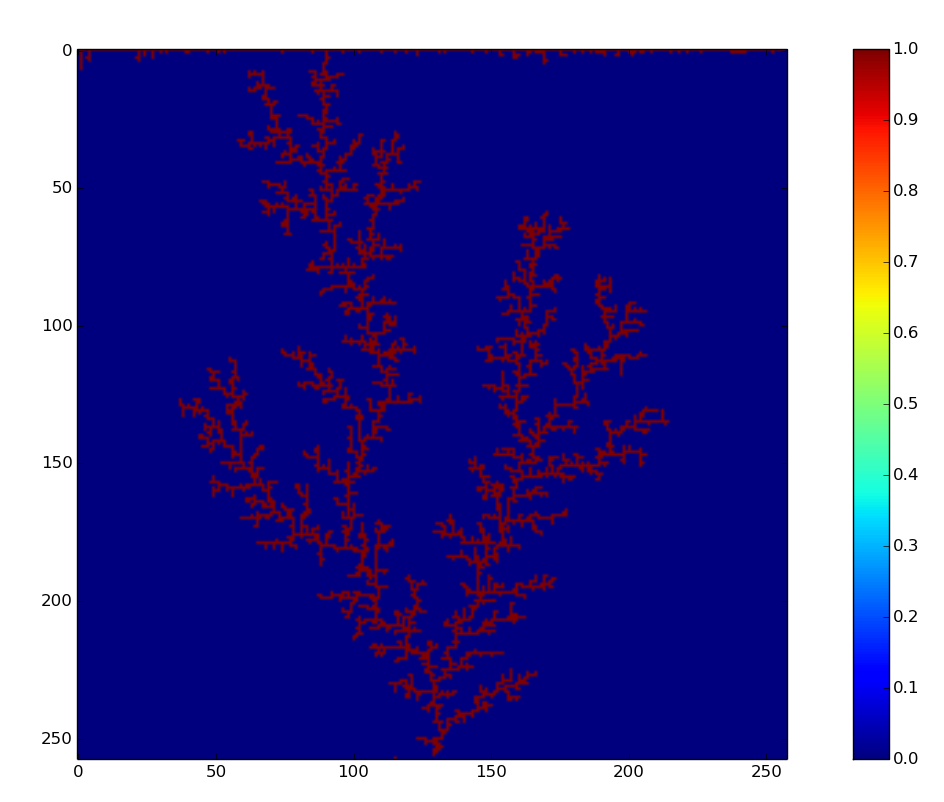
\includegraphics[width=\linewidth, trim={0cm 0cm 0cm 0cm},clip]{mcDLA_10.png} 
    \caption{$p_{stick} = 1$} 
    \label{fig:mcDLA_10} 
  \end{subfigure}%% 
  \begin{subfigure}[b]{0.5\linewidth}
    \centering
    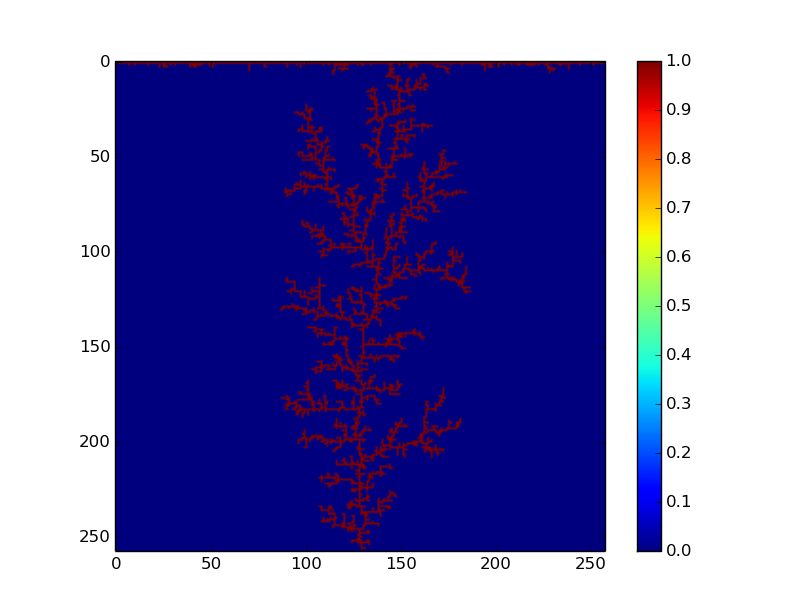
\includegraphics[width=\linewidth, trim={1cm 0.9cm 3.07cm 0cm},clip]{mcDLA_05.png}
    \caption{$p_{stick} = 0.5$} 
    \label{fig:mcDLA_05} 
  \end{subfigure}
  \begin{subfigure}[b]{0.5\linewidth}
    \centering
    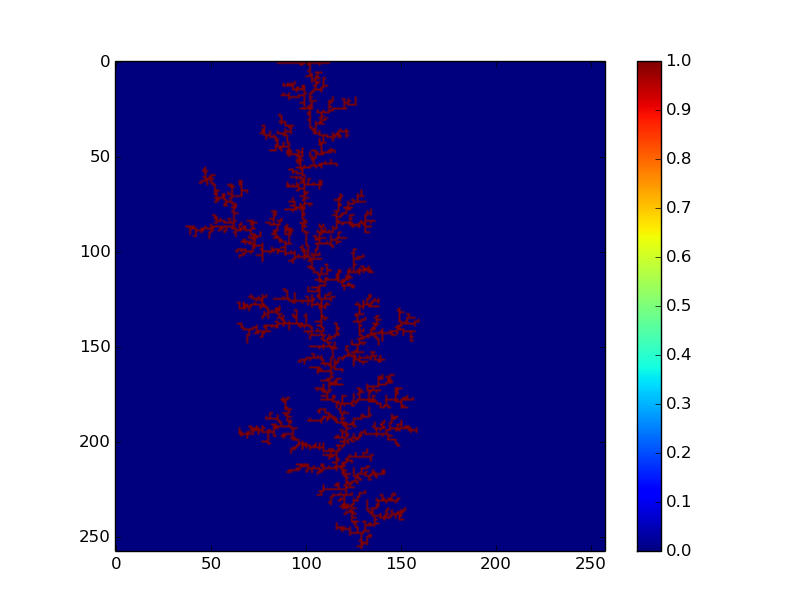
\includegraphics[width=\linewidth, trim={1cm 0.9cm 3.07cm 0cm},clip]{mcDLA_02.png}
    \caption{$p_{stick} = 0.2$} 
    \label{fig:mcDLA_02} 
  \end{subfigure}%%
  \begin{subfigure}[b]{0.5\linewidth}
    \centering
    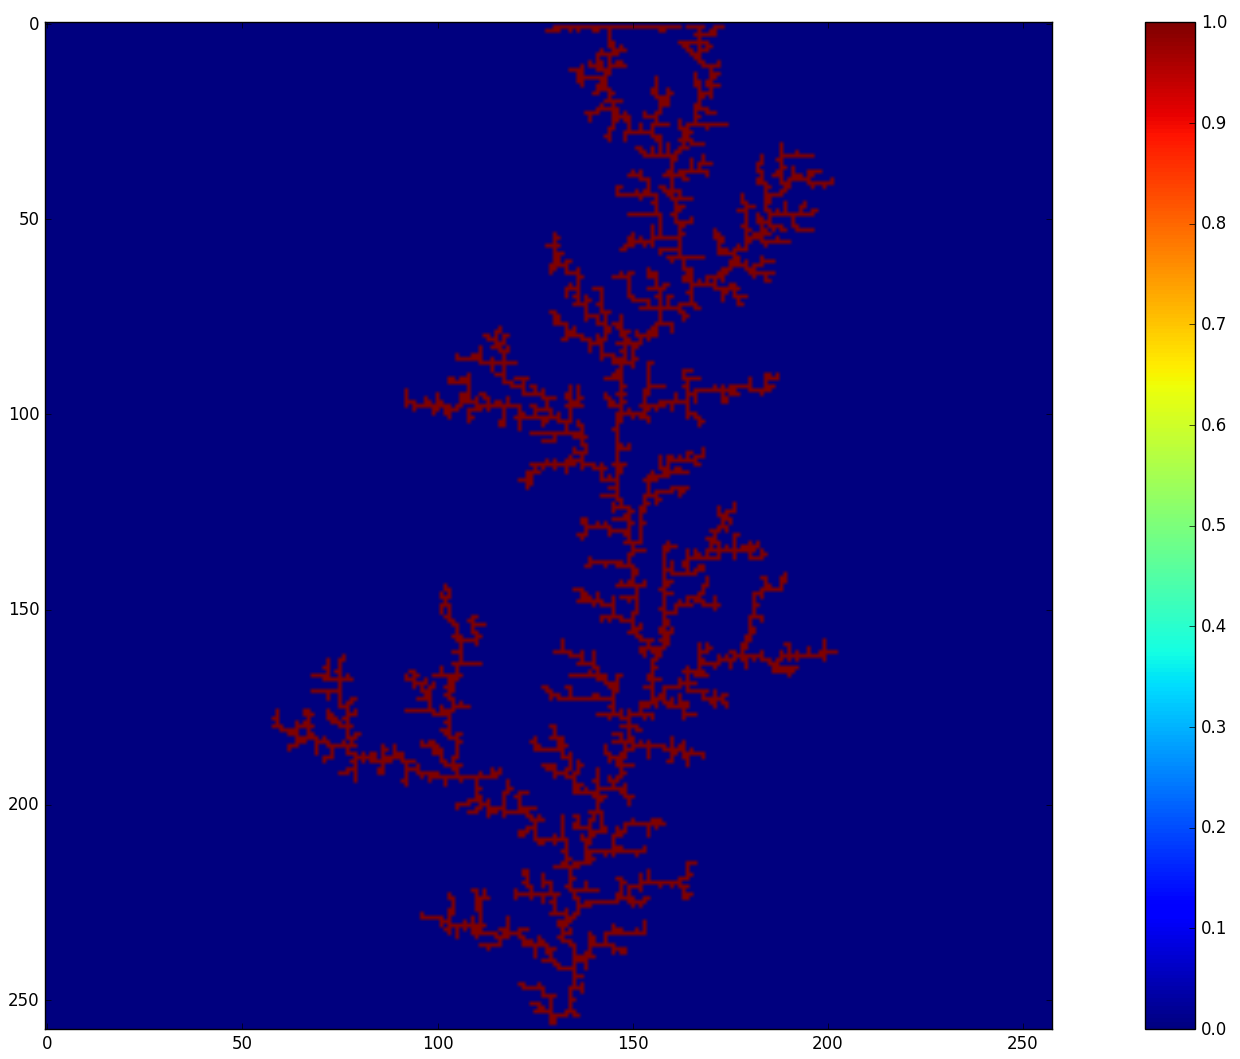
\includegraphics[width=5.6cm]{mcDLA_01.png}
    \caption{$p_{stick} = 0.1$} 
    \label{fig:mcDLA_01} 
  \end{subfigure}
  \caption{A Monte Carlo simulation of Diffusion Limited Aggregation for different values of the sticking probability $p_{stick}$. These structures can be compared to the structures in figure \ref{fig:DLA_eta10}-\ref{fig:DLA_eta20}}
  \label{fig:mcDLA} 
\end{figure}

\section{The Gray-Scott Model}
The Gray-Scott Model is a reaction-diffusion system. It models the flow of two chemicals, $u$ and $v$, by showing their concentrations over time as they diffuse and react with each other. Reaction-diffusion systems look like the familiar diffusion equation but they have an extra term that is a function of the relevant concentrations (e.g. $f(u, v)$). The Gray-Scott model can be expressed as:
\begin{equation} \label{eq:gray_scott}
\begin{aligned} 
    \frac{\partial u}{\partial t} &= D_u \nabla^2 u - uv^2 + f(1 - u),  \\
    \frac{\partial v}{\partial t} &= D_v \nabla^2 v + vv^2 - (f + k) v,
\end{aligned}
\end{equation}  
where $D_u$ and $D_v$ are the diffusion constants of the chemicals and $f$ and $k$ parameters of the underlying chemical reaction. To solve these partial differential equations for $u$ and $v$ we discretize the equations using finite difference methods. We divide 2D space in $N$ chunks of $\delta x$, $\delta y$ and time in periods of $\delta t$. In particular, we substitute 

\begin{align*}
    \frac{\partial u}{\partial t} &= \frac{u^{k+1}_i - u^k_i}{\delta t}, \\
    \begin{split}
        \nabla^2 u &= \left( \frac{\partial^2}{\partial x^2} + \frac{\partial^2}{\partial y^2} \right)^2 u, \\
        &= \frac{1}{\delta x^2} (u_{i+1,j} + u_{i-1,j} + u_{i,j+1} + u_{i,j-1} - 4 u_{i,j}),
    \end{split}
\end{align*}
in system \ref{eq:gray_scott} to get the discretization:
\begin{equation*} \label{eq:gray_scott_discrete}
\begin{aligned} 
    u^{k+1}_{i,j} &= u^k_{i,j} + \delta t \left(\frac{D_u}{\delta x^2} (u_{i+1,j} + u_{i-1,j} + u_{i,j+1} + u_{i,j-1} - 4 u_{i,j}) - uv^2 + f(1-u) \right) \\
    v^{k+1}_{i,j} &= v^k_{i,j} + \delta t \left(\frac{D_v}{\delta x^2} (v_{i+1,j} + v_{i-1,j} + v_{i,j+1} + v_{i,j-1} - 4 v_{i,j}) + uv^2 - (f + k) v \right)
\end{aligned}
\end{equation*}  

We take periodic boundary conditions along the $x$ and $y$ directions: $u(0, y, t) = u(N \delta x, y, t)$ and $u(x, 0, t) = u(x, N \delta y, t)$, with the same for $v$. We've implemented the derived discretization with these boundary conditions. 

For the parameters we've chosen $\delta t = \delta x = \delta y = 1$, $N=300$, $D_u = 0.16$, $D_v 0.08$, $f = 0.035$ and $k = 0.060$. Our initial conditions were $u = 0.5$ everywhere and $v = 0.25$ in a square around the origin and $v = 0$ elsewhere. We added a small amount of noise to the initial conditions of $u$ and $v$ of magnitude 0.05.

In figure \ref{fig:gs_time1} we see the concentrations of $u$ and $v$ over time. First at $t=0$ we see the square of the initial conditions with the added noise seen as speckles all over the domain. In the middle at $t=700$ we see that the noise has disappeared due to diffusion. The square itself has also disappeared, leaving behind four circles growing at its former corners. And at the bottom at $t=1300$ the circles have grown into four star-like shapes.

The process continues in figure \ref{fig:gs_time2}. The four stars have merged to a nice symmetric emblem. In the middle we see some breaking of symmetry, this could indicate the effect of numerical error, as the initial conditions were isotropic. Finally at the bottom the pattern has grown to extend over the boundaries. Because we implemented periodic boundary conditions, this final pattern can be used on tiles with the edges fitting perfectly.

\begin{figure}
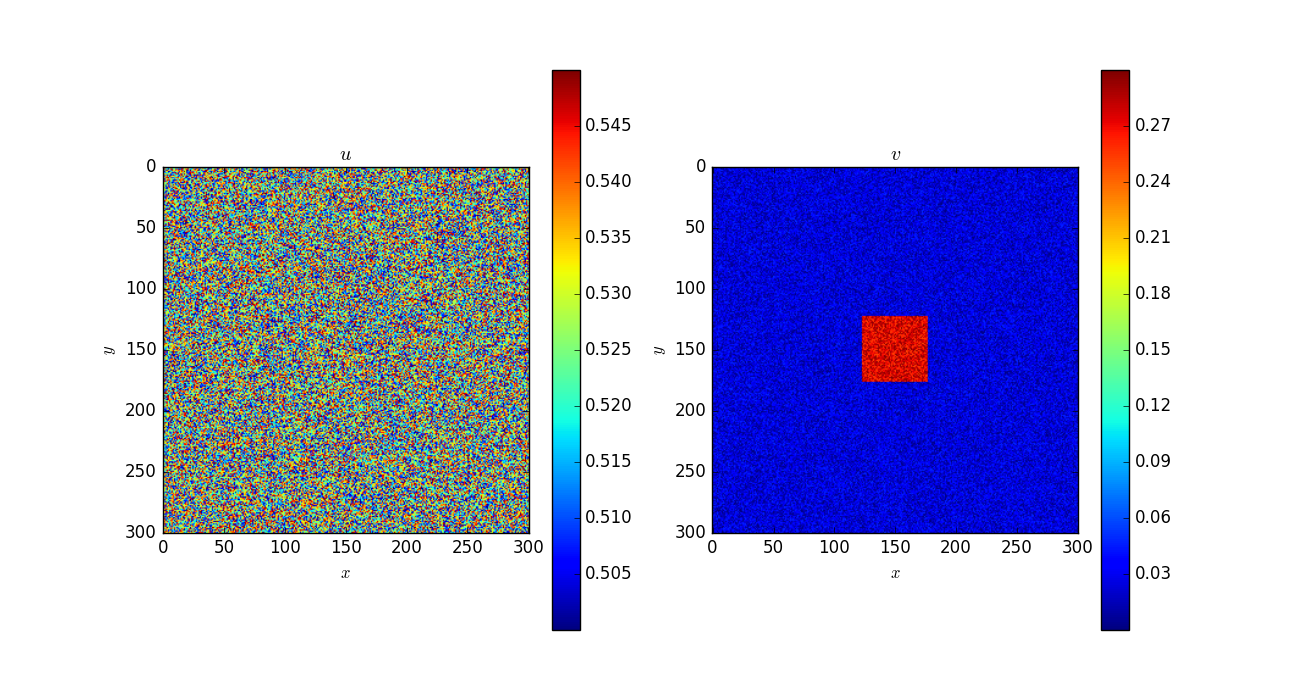
\includegraphics[width=12cm]{gs_0}
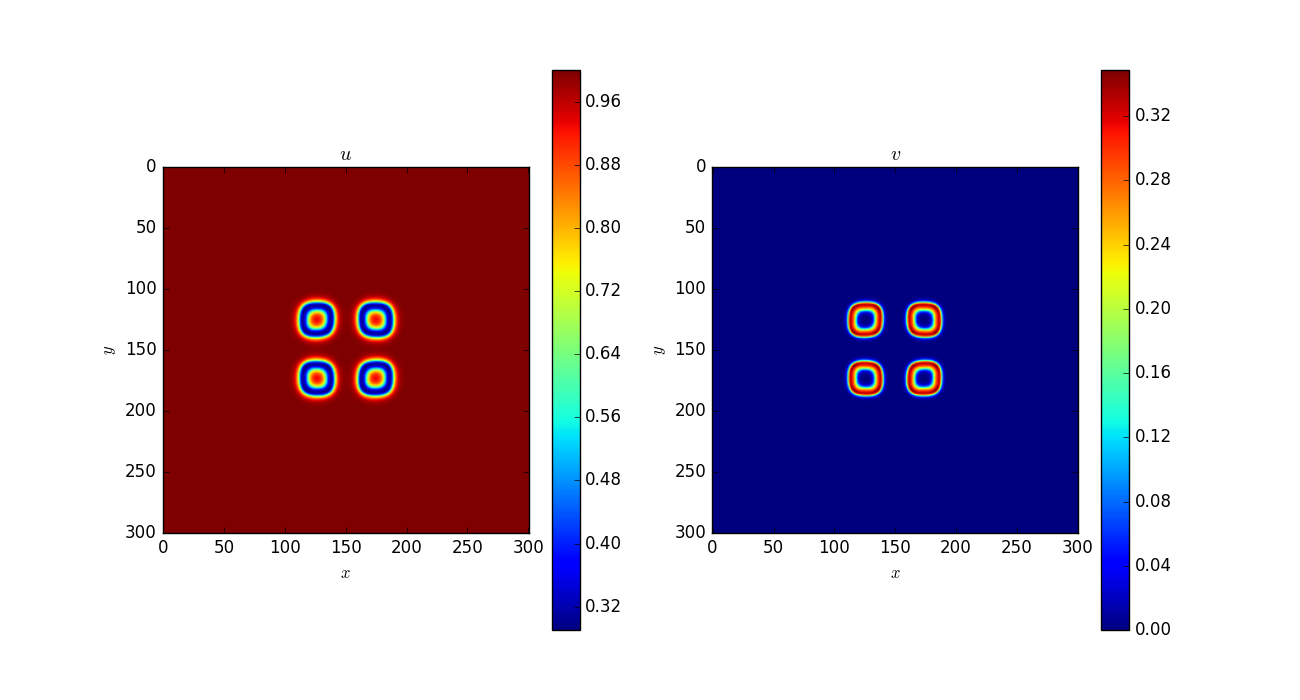
\includegraphics[width=12cm]{gs_700}
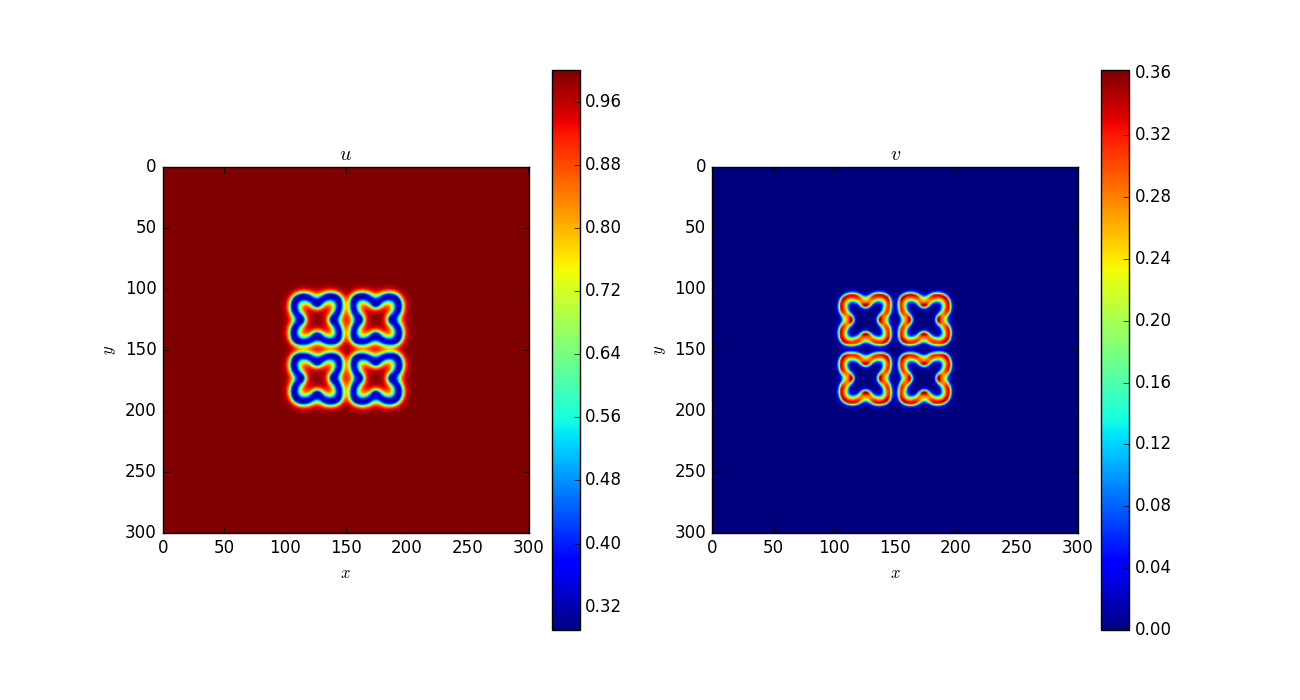
\includegraphics[width=12cm]{gs_1300}
\caption{The patterns that arise in the Gray-Scott model with the parameters described in the text. At the top we see the concentrations at time $t=0$, in the middle at $t=700$ and at the bottom at $t=1300$.}
\label{fig:gs_time1}
\end{figure}

\begin{figure}
    \centering
    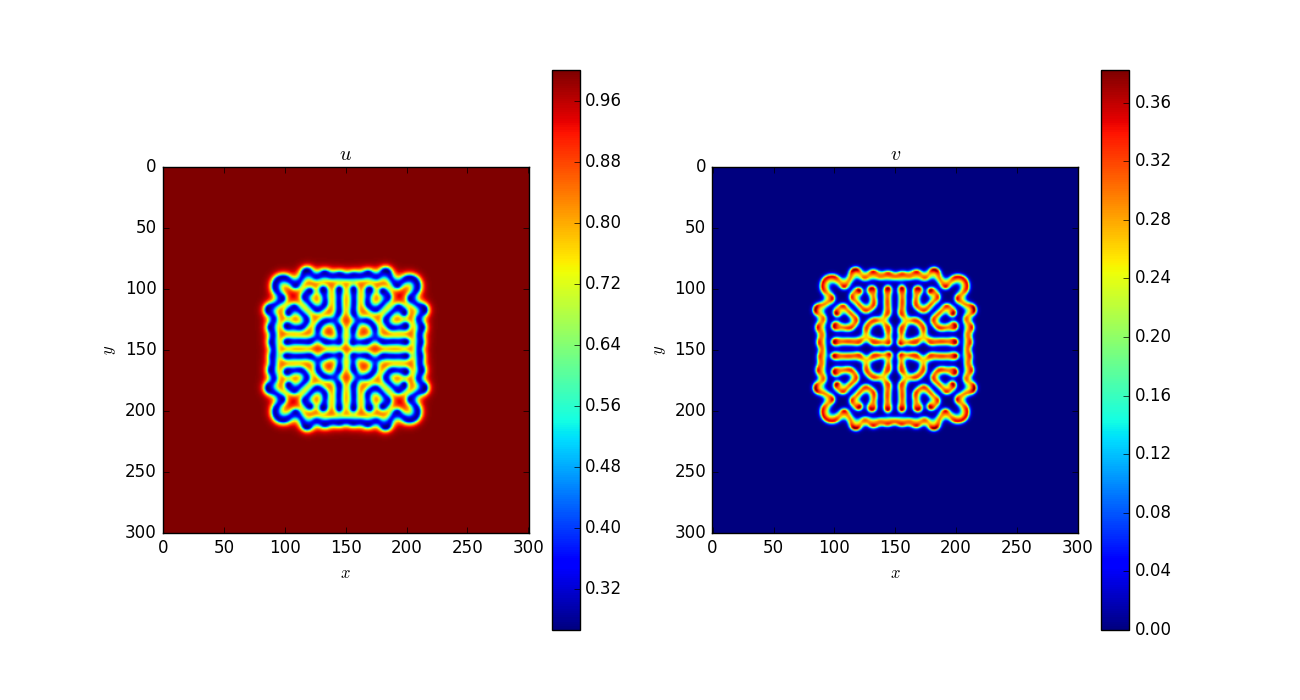
\includegraphics[width=12cm]{gs_2500}
    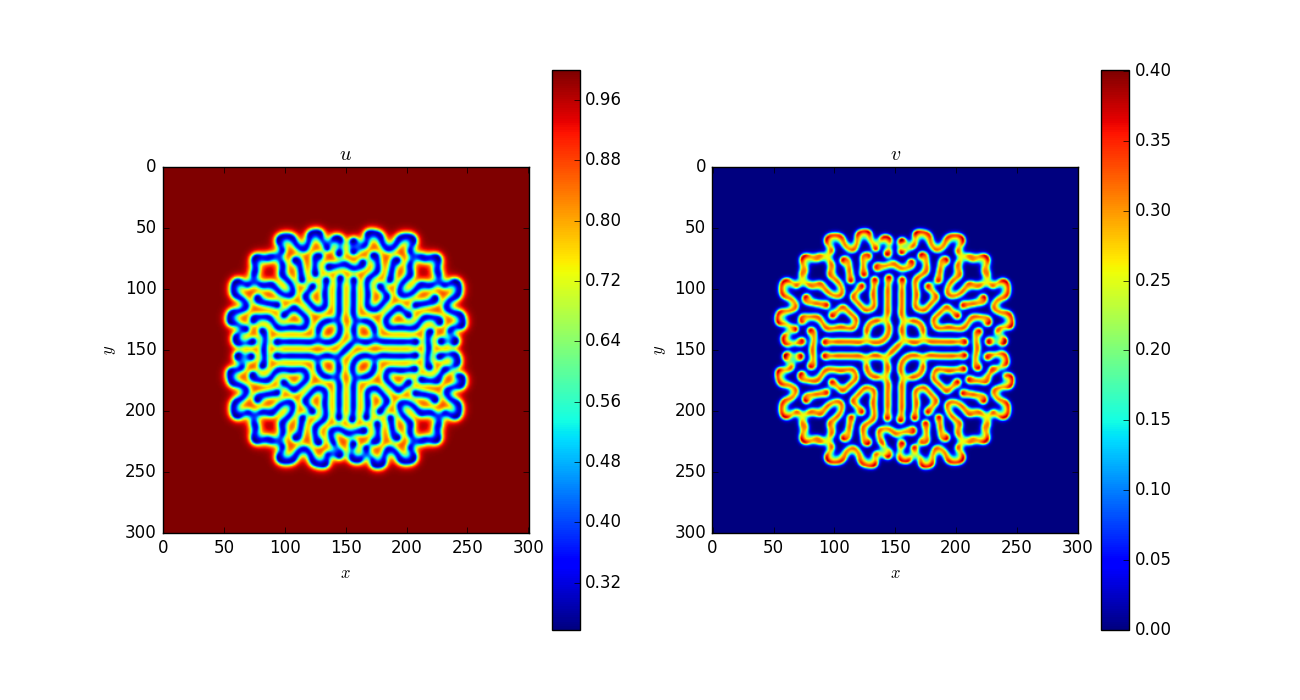
\includegraphics[width=12cm]{gs_4000}
    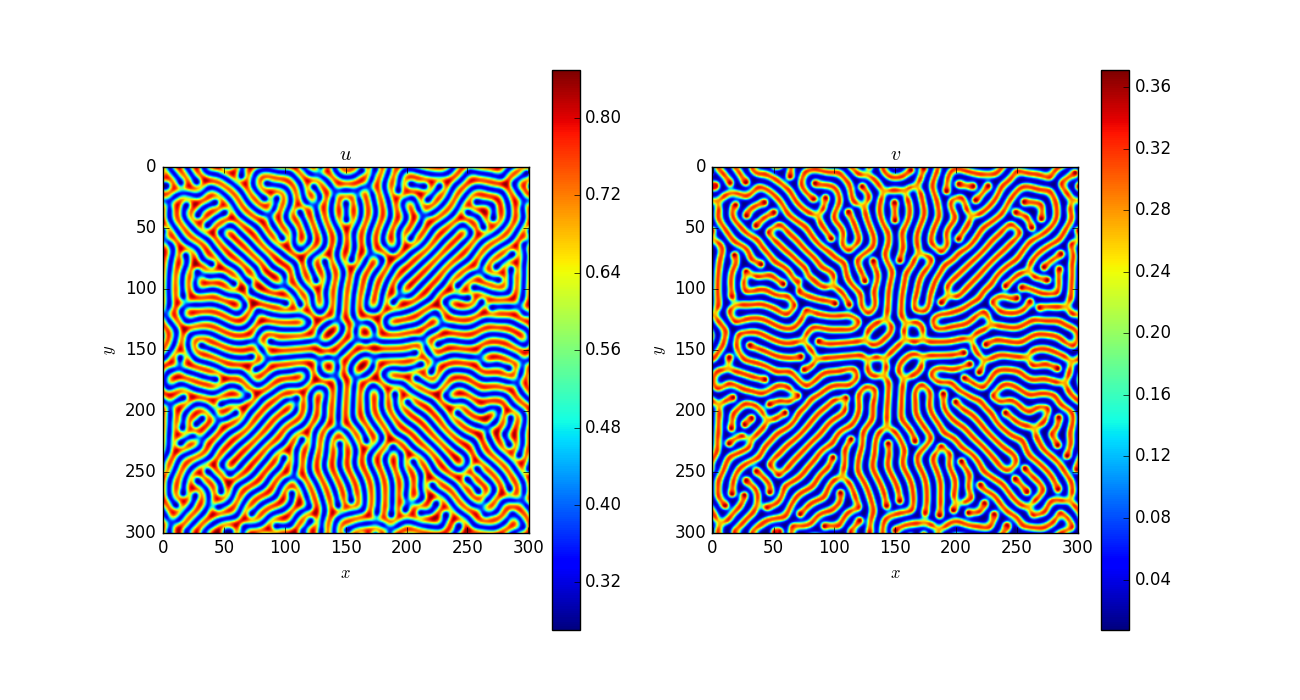
\includegraphics[width=12cm]{gs_10000}
    \caption{The continuation of figure \ref{fig:gs_time1}. Top: $t=2500$, middle: $t=4000$, bottom: $t=10000$.}
    \label{fig:gs_time2}
\end{figure}

We now explore the patterns formed when the parameters are changed slightly: $f=0.030$ and $k=0.055$. Everything else is the same. This time we omit $u$ from the plots, because it does not add new information on the patterns given $v$. In figure \ref{fig:gs2} we see the formation of the patterns. The initial square grows into a waffle (b and c) and continues expanding until we end up with many small mountains (f), or spots. We conclude by noting that the small change in parameters lead to quite different patterns.

\begin{figure}[ht]
  \begin{subfigure}[b]{0.5\linewidth}
    \centering
    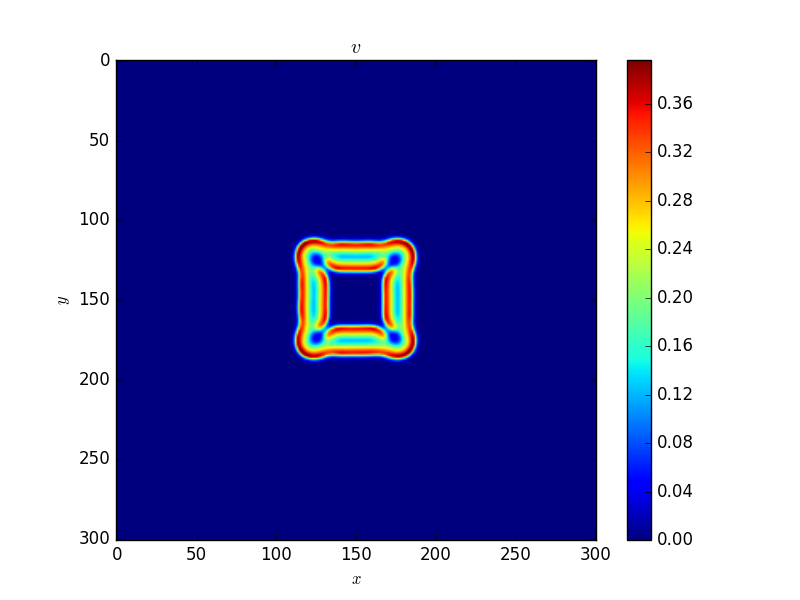
\includegraphics[width=7cm]{gs2_350}
    \caption{$t = 350$}
    \label{fig:gs2_350}
  \end{subfigure}%%
  \begin{subfigure}[b]{0.5\linewidth}
    \centering
    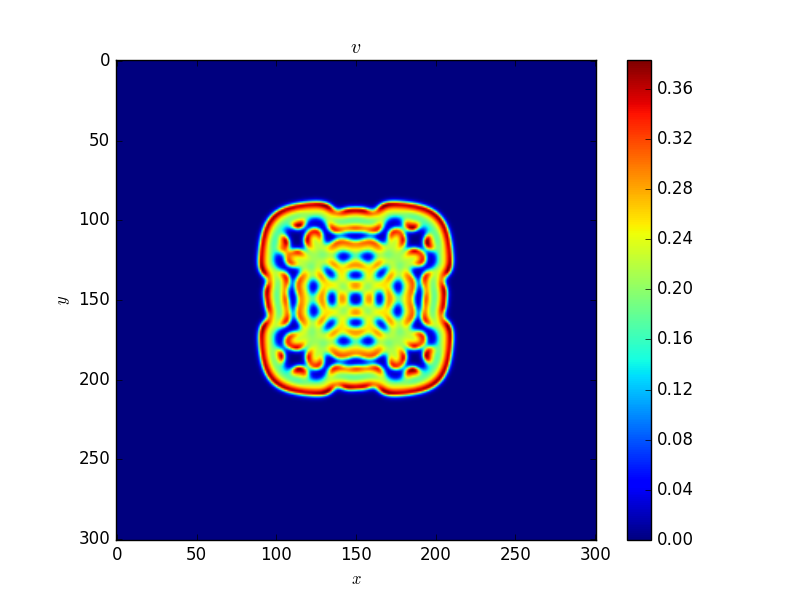
\includegraphics[width=7cm]{gs2_1000}
    \caption{$t = 1000$}
    \label{fig:gs2_1000}
  \end{subfigure}
  \begin{subfigure}[b]{0.5\linewidth}
    \centering
    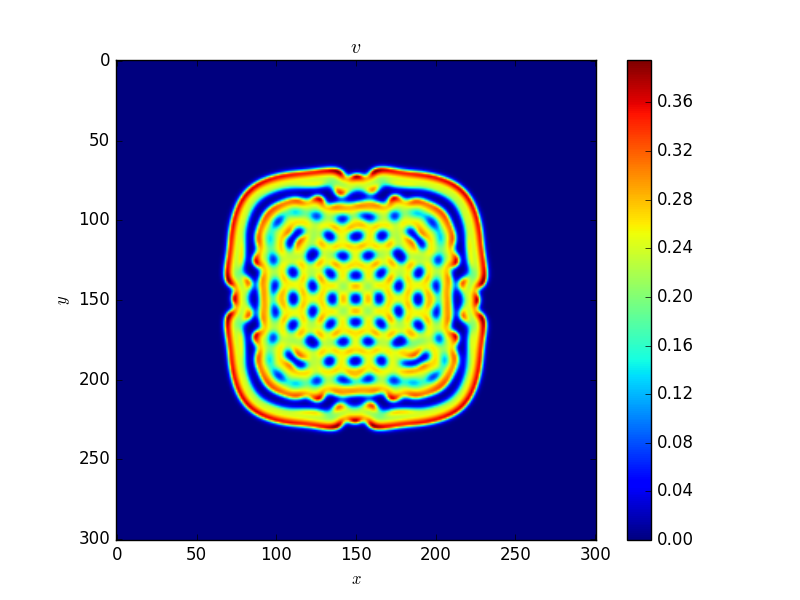
\includegraphics[width=7cm]{gs2_1600}
    \caption{$t = 1600$}
    \label{fig:gs2_1600}
  \end{subfigure}%%
  \begin{subfigure}[b]{0.5\linewidth}
    \centering
    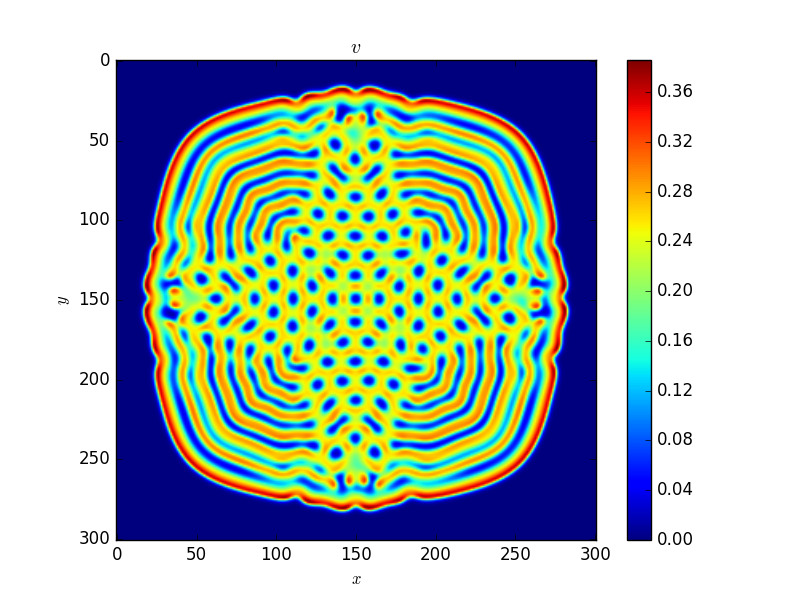
\includegraphics[width=7cm]{gs2_3000}
    \caption{$t = 3000$}
    \label{fig:gs2_3000}
  \end{subfigure}
  \begin{subfigure}[b]{0.5\linewidth}
    \centering
    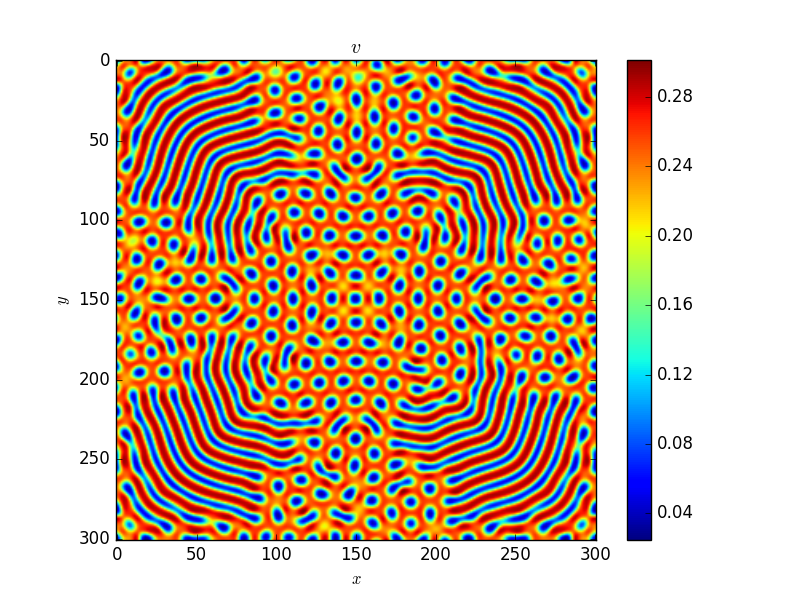
\includegraphics[width=7cm]{gs2_5000}
    \caption{$t = 5000$}
    \label{fig:gs2_5000}
  \end{subfigure}%%
  \begin{subfigure}[b]{0.5\linewidth}
    \centering
    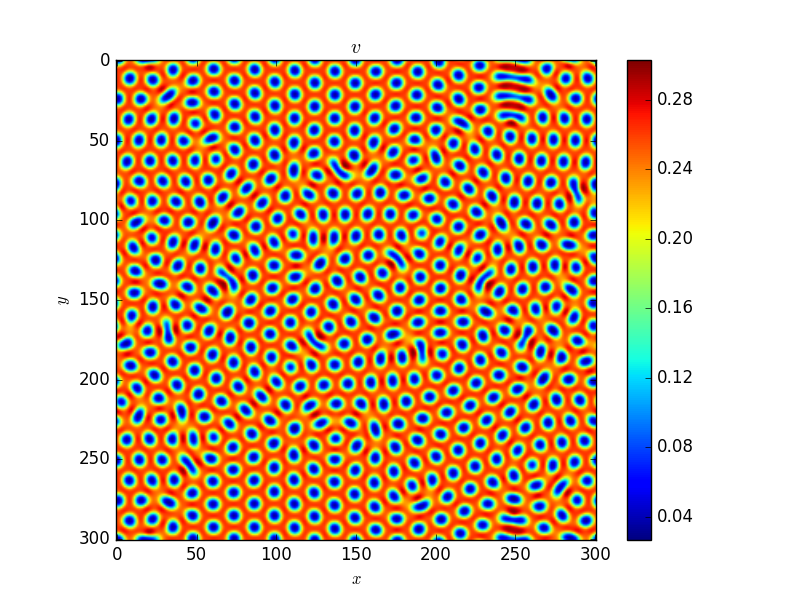
\includegraphics[width=7cm]{gs2_50000}
    \caption{$t = 50000$}
    \label{fig:gs2_50000}
  \end{subfigure}
  \caption{The Gray-Scott model with $f=0.030$ and $k=0.055$.}
  \label{fig:gs2}
\end{figure}

\bibliography{references}
\bibliographystyle{unsrt}

\end{document}
